\documentclass[a4paper,11pt]{article}

%
% PDFファイルの作成方法
%
% ・dvipdfmを使う場合
%   dvipdfm -p A4 sample.dvi
%
% ・Adobe Acrobat (Distiller) を使う場合
%   dvipsk -D 600 -t a4 -P pdf sample.dvi
%   psファイルをDistillerでpdfへ変換
%

% ***************
%      注意!
% ***************
% 以下のtxfontsパッケージを使用するとcmフォントが(数式も含めて)Times,
% Helveticaなどに置き換えられます。詳しくは下記のウェブページなどをご参照くださ
% い。
% http://oku.edu.mie-u.ac.jp/~okumura/texwiki/?TXFonts
%
% これを使いたくない方は以下の\usepackage{txfonts}を無効にしてください。
% その場合にはcmフォントがPDFに埋め込まれるのでファイルサイズが多少大きくなります。
\usepackage{txfonts}
\usepackage{url}
\usepackage[notes,backend=biber]{biblatex-chicago}
\usepackage{listings}
\bibliography{references}
% \usepackage{xeCJK}
% \usepackage{CJKutf8}
\usepackage{graphicx}
\graphicspath{{images/}}

% 
% マージン設定(できるだけ変更しないでください)
%
\setlength{\oddsidemargin}{0truemm}
\setlength{\hoffset}{-0.4truemm}
\setlength{\voffset}{-0.4truemm}
\setlength{\textheight}{247truemm}
\setlength{\textwidth}{160truemm}
\setlength{\headheight}{0truemm}
\setlength{\topmargin}{0truemm}
\setlength{\headsep}{0truemm}

\pagestyle{empty}

\begin{document}
\renewcommand{\baselinestretch}{1.20}\small\normalsize

\begin{center}
%   \textbf{\Large 応用物理学会学術講演会予稿のタイトル}
  
  \textbf{\large Leveraging Segmentation of Physical Units through a Newly Open Source Corpus}
  
  \textbf{Luca Foppiano, Akira Suzuki, Thaer M. Dieb, Masashi Ishii\footnote{Corresponding author: ISHII.Masashi@nims.go.jp} and Mikiko Tanifuji}
  
  \textbf{MaDIS, National Institute for Materials Science (NIMS)}
%   \textbf{Research and Services Division of Materials Data and Integrated System (MaDIS), National Institute for Materials Science (NIMS), 1-1 Namiki, Tsukuba, Ibaraki 305-0044, Japan}
  
   \textbf{E-mail: FOPPIANO.Luca@nims.go.jp}
\end{center}

%0.2\cdot e\textsuperscript{3}$

%The ability to correctly parse and normalise physical measurements is a task common in almost every domain. 
The identification of physical measurements is a recurrent need in materials informatics (MI). For example, the extraction of superconductor materials and their properties\footcite{foppiano2019proposal} requires to identify and understand temperature, pressure, magnetisation.
When designing automatic systems for information extraction from scientific literature, the identification of the raw measurement alone is not sufficient. Quantity transformations, such as normalisation, require the understanding of values and units, which are contained in unstructured text with ad-hoc conventions. 
%In polymers, the standard unit does not correspond with the one in the Polynfo reference database (e.g. \textit{specific volume} is standardised as  \( \frac{m\textsuperscript{3}}{kg} \) but is represented in Polynfo with \( \frac{cm\textsuperscript{3}}{kg} \).
%It is common to encounter new variations or complex units not present in any general dictionaries. 
String matching and lookups are failing with growing unit complexity and variability. Therefore a generic unit segmentation system is necessary.

This contribution is part of a larger project called Grobid-quantities \footcite{grobid-quantities}, a machine learning (ML) based, Open Source system for extracting and normalising physical measurements from scientific and patent literature. 
%Grobid-quantities is a module based on Grobid \autocite{GROBID}, a machine learning framework for parsing and structuring PDF documents. 
In this submission, we present a general approach for units representation, and we introduce the public availability (Creative Commons licence) of a corpus of segmented physical units. 
%Corpora of this kind are needed for training newly sequence labelling unit segmentation models or to evaluate existing systems. 
% There are several work related on extraction of physical units. \textit{Berrahou et all}\autocite{berrahou2013extract} illustrates a fairly similar model for unit representation without taking in account the needs of unit normalisation. \textit{Peter et all}\autocite{peter2017quantity} describes the construction of a database of units using machine learning. Unfortunately they do not provide the resulting database publicly. 
Currently, there are no comparable results in scientific literature because no public datasets are available for this task.
Our approach for the unit representation follows the International System of Measurement (SI), where each unit is represented as a product of triples: \textit{prefix}, \textit{base} and \textit{power}. This straightforward approach offers the flexibility to support any combination of units from any system of measurements. 
%For example \texttt{kV/cm\textsuperscript{2}}, corresponds to \texttt{$kV\cdot cm\textsuperscript{-2}$} and becomes \texttt{[(k, V, 1), (c, m, -2)]} as product of triples. 
%The example previously illustrated is then encoded in XML as \texttt{\small{<unit><prefix>k</prefix><base>V</base> <pow>\char`/</pow><prefix>c</prefix><base>m</base><pow>2<pow></unit>}}.  
Figure~\ref{fig:dataset example} illustrates an example where \texttt{µg/ml} is tokenised and segmented as product of triples.
\begin{figure}[h]
    \centering
    % 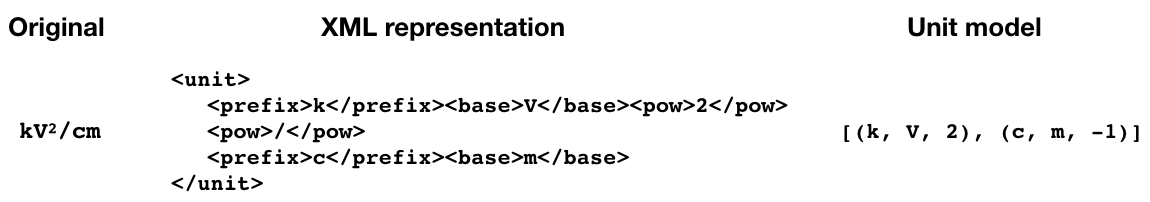
\includegraphics[width=0.9\textwidth,natwidth=575,natheight=101]{sample-corpus.png}
    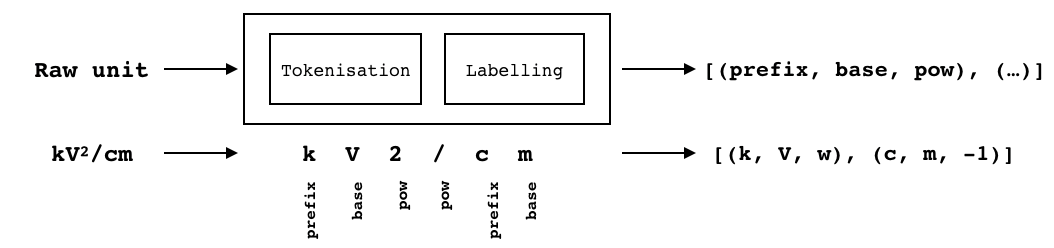
\includegraphics[width=0.9\textwidth,natwidth=527,natheight=124]{system-schema.png}
    \caption[] {The process of parsing a raw unit into the product of triples. Notice that the label \texttt{pow} is used to identify both exponent and division marks (needed to correctly set the second triple's exponent, in this case negative).}
    \label{fig:dataset example}
\end{figure}

We used the Grobid-quantities ML-based unit segmentation implementation to create a new corpus. We used data provided by previous work of some of the authors\footcite{suzuki2018constructing}, where about 2000 units were extracted from 3490 papers of Journal of Applied Physics. The data was pre-annotated and manually corrected. 

The resulting corpus contains approximately 700 simple and 1300 complex units, and it's available in XML format at the Grobid-quantities repository\footnotemark[3]. It is suitable for evaluating new or existing systems for unit segmentation. We plan to increase the coverage by adding new data from other domains.

\end{document}